\RequirePackage{luatex85}
\documentclass[english,aps,prd,preprint,showpacs,superscriptaddress,groupedaddress,fixfloats]{revtex4-1}

% --------------------------------Package--------------------------------------
	\usepackage{parskip}
	\usepackage{physics}
	\usepackage{amsmath}
	\usepackage{amssymb}
	\usepackage{xcolor}
	\usepackage[colorlinks,breaklinks=true]{hyperref}
	\usepackage{array}
	\usepackage{longtable}
	\usepackage{multirow}
	\usepackage{comment}
	\usepackage{graphicx}
	\usepackage{amsfonts}
	\usepackage{bm}
	\usepackage{slashed}
	\usepackage{dsfont}
	\usepackage{mathtools}
	\usepackage[compat=1.1.0]{tikz-feynman}
	\usepackage{makecell}
	\usepackage{mathrsfs}
	\usepackage{xparse}
	\usepackage{enumerate}
	\usepackage{mathtools}

	%\usepackage{authblk}
	\usepackage[T1]{fontenc}
	%\usepackage{apacite}
	%\usepackage[nottoc]{tocbibind}
	%\usepackage[utf8]{inputenc}
	\usepackage[caption=false]{subfig}
	
% ---------------------------------END-----------------------------------------



% ---------------------------------Xiong's-------------------------------------
	\usepackage{esint}
	%\usepackage{ulem}
	\usepackage{bbm}
	\usepackage{babel}
	\usepackage{footmisc}


	\newcommand{\nn}{\nonumber}
	\newcommand{\lc}{\lowercase}
	% \newcommand{\beq}{\begin{equation}}
	% \newcommand{\eeq}{\end{equation}}
	% \newcommand{\bqa}{\begin{eqnarray}}
	% \newcommand{\eqa}{\end{eqnarray}}
	% \newcommand {\bseq}{\begin{subequations}}
	% \newcommand {\eseq}{\end{subequations}}
	\newcommand {\pvint}[2]{{\int\!\!\!\!\!\!-}_{\!\!\!\!#1}^{#2}}
	\newcommand*{\rom}[1]{\uppercase\expandafter{\romannumeral #1\relax}}
	%\newcommand{\nn}{\nonumber}
	%\begin{comment}
			\def\Xint#1{\mathchoice
			{\XXint\displaystyle\textstyle{#1}}%
			{\XXint\textstyle\scriptstyle{#1}}%
			{\XXint\scriptstyle\scriptscriptstyle{#1}}%
			{\XXint\scriptscriptstyle\scriptscriptstyle{#1}}%
			\!\int}
			\def\XXint#1#2#3{{\setbox0=\hbox{$#1{#2#3}{\int}$ }
			\vcenter{\hbox{$#2#3$ }}\kern-.6\wd0}}
			\def\ddashint{\Xint=}
			\def\dashint{\Xint-}
	%\end{comment}

    % \graphicspath{{./figs/}}
% ---------------------------------END-----------------------------------------

% ---------------------------CustomCommand-------------------------------------
    \newcommand{\numberthis}{\addtocounter{equation}{1}\tag{\theequation}}

	\newcommand{\red}[1]{{\color{red}#1}}
	
	\newcommand{\mm}[1]{\frac{\dd^4#1}{(2\pi)^4}}
	\newcommand{\mme}[1]{\frac{\dd^3\vb{#1}}{(2\pi)^3}}
	\newcommand{\mmd}[2][d]{\frac{\dd^{#1}{#2}}{(2\pi)^{#1}}}

% ---------------------------------END-----------------------------------------

% ------------------------------mathtools---------------------------------------
	\newcommand\MTkillspecial[1]{% helper macro
		\bgroup
		\catcode`\&=9
		\let\\\relax%
		\scantokens{#1}%
		\egroup
		}
	\DeclarePairedDelimiter\BraceM\{\}
	\reDeclarePairedDelimiterInnerWrapper\BraceM{star}{
		\mathopen{#1\vphantom{\MTkillspecial{#2}}\kern-\nulldelimiterspace\right.}
		#2
		\mathclose{\left.\kern-\nulldelimiterspace\vphantom{\MTkillspecial{#2}}#3}
		}
	\let\Bqty\relax
	\newcommand{\Bqty}[1]{\BraceM*{#1}}

	\DeclarePairedDelimiter\ceil{\lceil}{\rceil}
	\DeclarePairedDelimiter\floor{\lfloor}{\rfloor}

	% \DeclarePairedDelimiter{\TRM}{\tr\{}{\}}
	% \reDeclarePairedDelimiterInnerWrapper\TRM{star}{
	% 	\mathopen{#1\vphantom{\MTkillspecial{#2}}\kern-\nulldelimiterspace\right.}
	% 	#2
	% 	\mathclose{\left.\kern-\nulldelimiterspace\vphantom{\MTkillspecial{#2}}#3}
	% 	}
	% \renewcommand{\tr}[1]{\TRM*{#1}}
% ---------------------------------END-----------------------------------------


% --------------------------------LuaLaTeX Fonts--------------------------------
    %\setmainjfont[BoldFont=FandolSong-Bold]{FandolSong-Regular}
    %\setsansjfont{FandolSong-Bold}
    %\setlength{\parindent}{2em}
    %\linespread{1.2}
    %\renewcommand\Authsep{, }	
% ----------------------------------END-----------------------------------------



%\allowdisplaybreaks

% ===============================titlesec=======================================
    \usepackage{titlesec}
    \titleformat{\paragraph}[runin]{\itshape}{}{}{}[]
    \titlespacing*{\paragraph}{0pt}{*}{*}
% ==============================================================================

% ==============================================================================
% Tikz-Feynman Externalization
% ==============================================================================
\usepackage{shellesc}
\usetikzlibrary{external}
% \usepgfplotslibrary{external}
\tikzexternalize[shell escape=-enable-write18,prefix=./,system call={lualatex \tikzexternalcheckshellescape -halt-on-error -interaction=batchmode -jobname "\image" "\texsource"},up to date check=diff]

\makeatletter
\newcommand{\pushright}[1]{\ifmeasuring@#1\else\omit\hfill$\displaystyle#1$\fi\ignorespaces}
\newcommand{\pushleft}[1]{\ifmeasuring@#1\else\omit$\displaystyle#1$\hfill\fi\ignorespaces}
\makeatother

\setlength{\parindent}{2ex}




\begin{document}

% ------------------------------------------------------------------------------
% Title, authors and institutes
% ------------------------------------------------------------------------------

\title{Coulomb Resummation Near $t \bar t$ Threshold in $e^+e^-\to HZ$ Process}

\author{Yingsheng Huang}
\email{huangys@ihep.ac.cn}
\affiliation{Institute of High Energy Physics, Chinese Academy of
	Sciences, Beijing 100049, China\vspace{0.2 cm}}
\affiliation{School of Physics, University of Chinese Academy of Sciences,
	Beijing 100049, China\vspace{0.2 cm}}

% \author{Yu Jia}
% \email{jiay@ihep.ac.cn}
% \affiliation{Institute of High Energy Physics, Chinese Academy of
% 	Sciences, Beijing 100049, China\vspace{0.2 cm}}
% \affiliation{School of Physics, University of Chinese Academy of Sciences,
% 	Beijing 100049, China\vspace{0.2 cm}}
% %\affiliation{Center for High Energy Physics, Peking University, Beijing 100871,
% %	China}

% \author{Rui Yu}
% \email{yurui@ihep.ac.cn}
% \affiliation{Institute of High Energy Physics, Chinese Academy of Sciences, Beijing 100049, China\vspace{0.2 cm}}
% \affiliation{School of Physics, University of Chinese Academy of Sciences,
% 	Beijing 100049, China\vspace{0.2 cm}}

\date{\today}
% ------------------------------------------------------------------------------
% End
% ------------------------------------------------------------------------------

%%%%%%%%%%%%%%%%%%%%%%%%%%%%%%%%%%%%%%%%%%%%%%%%%%%%%%%%%%%%%%%%%%%%%%%%%%%%%%
\begin{abstract}

\end{abstract}
%%%%%%%%%%%%%%%%%%%%%%%%%%%%%%%%%%%%%%%%%%%%%%%%%%%%%%%%%%%%%%%%%%%%%%%%%%%%%%
%\pacs{}

\maketitle

\section{Introduction}
The first relevant calculation should be Fadin et al. in 1987 \cite{Fadin1987}. The imaginary part of the Coulomb Green function is given explicitly. The whole expression is given by Melnikov et al. in 1994 \cite{Melnikov:1994jb}. While this being true, there's a real constant $D$ related to renormalization scheme that remains to be fixed. In 1991, Strassler and Peskin details the top quark production near threshold at the leading order in $\alpha_s$. The high order correction effects considered are restrict to running $\alpha_s$ (to two loop order), Higgs static potential and electroweak correction though. Kats and Schwartz gave a review about annihilation decays of bound states at LHC \cite{Kats:2009bv}. There're also a number of papers involving the threshold effects of diphoton resonance\cite{}, in which Chway et al. explicitly expressed that the 1-loop amplitude can be well separated into relativistic and non-relativistic parts near the threshold. 
For exclusive processes, 

\section{Coulomb Part}
We have two diagrams:
\begin{align*}
	\begin{tikzpicture}[baseline=(g2.base)]
		\begin{feynman}
			\diagram[horizontal=g1 to g2]{
			e1[particle=\(e^-\)] --[fermion] g1 --[fermion] e2[particle=\(e^+\)];
			g1 --[photon, edge label=\(\gamma*/Z\)] g2;
			g2 --[fermion] t1 --[boson] z[particle=\(Z\)];
			g2 --[anti fermion] t2 --[scalar] h[particle=\(H\)];
			t1 --[fermion,edge label=\(t\)] t2;
			};
		\end{feynman}
	\end{tikzpicture}
	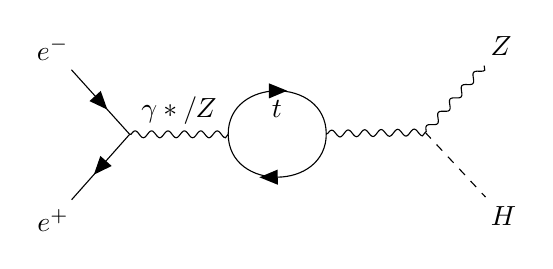
\begin{tikzpicture}[baseline=(g2.base)]
		\begin{feynman}
			\diagram[horizontal=g1 to g2]{
			e1[particle=\(e^-\)] --[fermion] g1 --[fermion] e2[particle=\(e^+\)];
			g1 --[photon, edge label=\(\gamma*/Z\)] g2;
			g2 --[fermion, half left, edge label'=\(t\)] t1 --[boson] z1;
			g2 --[anti fermion, half right] t1 --[draw=none] z1;
			z1 --[scalar] h[particle=\(H\)];
			z1 --[boson] z[particle=\(Z\)];
			};
		\end{feynman}
	\end{tikzpicture}
\end{align*}
The leading order Coulomb resummation (which refers to Coulomb resummation in the following since no higher order correction is involved) can be expressed diagrammatically as
\begin{align*}
	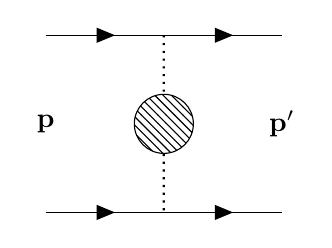
\begin{tikzpicture}
		\begin{feynman}
			\diagram[horizontal=t1 to t3, layered layout]{
			t1 --[fermion] t2 --[fermion] t3;
			t4 --[fermion] t5 --[fermion] t6;
			{[same layer] t2 --[draw=none] t5};
			};
			\node[blob] at ($(t2)!0.5!(t5)$) (c);
			\diagram*{
			(t2) --[ghost] (c);
			(c) --[ghost] (t5);
			};
			\node at ($(t1)!0.5!(t4)$) (p) {\(\vb{p}\)};
			\node at ($(t3)!0.5!(t6)$) (p) {\(\vb{p}'\)};
		\end{feynman}
	\end{tikzpicture}
\end{align*}
where the blob stands for the resummation of all Coulomb-mode gluon exchange. This Green function can be expressed as (including the diagram without Coulomb-gluon exchange) $G(\vb{p},\vb{p}';E)= G_0^{(1)}(\vb{p},\vb{p}';E)$ which obeys a Lippmann-Schwinger equation\cite{Beneke:2013jia}
\begin{align}
	\left(\frac{\mathbf{p}^{2}}{m}-E\right) G_{0}^{(R)}\left(\mathbf{p}, \mathbf{p}^{\prime} ; E\right)+\tilde{\mu}^{2 \epsilon} \int \frac{d^{d-1} \mathbf{k}}{(2 \pi)^{d-1}} \frac{4 \pi D_{R} \alpha_{s}}{\mathbf{k}^{2}} G_{0}^{(R)}\left(\mathbf{p}-\mathbf{k}, \mathbf{p}^{\prime} ; E\right) =(2 \pi)^{d-1} \delta^{(d-1)}\left(\mathbf{p}-\mathbf{p}^{\prime}\right).
\end{align}
In our case, it's a color-singlet state, thus $D_1=-C_F=\frac{4}{3}$. The coordinate space Coulomb Green function $G\left(\mathbf{r}, \mathbf{r}^{\prime}; E\right)$ is related to $G(\vb{p},\vb{p}';E)$ via a Fourier transform
\begin{align}
	G(\mathbf{p},\vb{p}' ; E)=\int \mathrm{d}^{3} \mathbf{r}\dd^3 \vb{r}' G\left(\mathbf{r}, \mathbf{r}^{\prime}; E\right) e^{-\mathrm{i} \mathbf{p}\cdot \mathrm{r}}e^{-\mathrm{i} \mathbf{p}' \cdot\mathrm{r}'}
\end{align}
and $G\left(\mathbf{r}, \mathbf{r}^{\prime}; E\right)$ which obeys a Schr\"odinger equation
\begin{align}
	\left(-\frac{\nabla_{(r)}^{2}}{m}+\frac{D_{R} \alpha_{s}}{r}-E\right) G\left(\mathbf{r}, \mathbf{r}^{\prime} ; E\right)=\delta^{(3)}\left(\mathbf{r}-\mathbf{r}^{\prime}\right)
\end{align}
What we want is actually a spatially local Green function $G(0,0;E)$, of which the result is given\cite{Fadin1987,Melnikov:1994jb}
\begin{align}
	G(0,0 ; E)=-\frac{m_{t} p}{4 \pi}+\frac{m_{t} p_{0}}{2 \pi} \log \left(\frac{m_{t}}{p} D\right)+\frac{m_{t} p_{0}^{2}}{2 \pi} \sum_{n=1}^{\infty} \frac{1}{n\left(n p-p_{0}\right)}
\end{align}
where $D$ is a real constant depends on renormalization scheme and is taken to be unity here (if we're to pursuit two-loop precision, this constant must be determined by fixed order calculation), $p_0=\frac{2}{3}m_t\alpha_s$ and $p=\sqrt{m_t\left( -E-i\epsilon \right)}$. Considering
\begin{align}
	\sum_{i=1}^{n} \frac{1}{n\left(n p-p_{0}\right)}=-\frac{\psi^{(0)}\left(1-\frac{p_{0}}{p}\right)+\gamma_E}{p_{0}}=-\frac{H_{-p_{0}/p}}{p_{0}}
\end{align}
where $H_n=\sum_{i=1}^n\frac{1}{i}$ is the harmonic number, the Coulomb Green function becomes
\begin{align}
	G(0,0 ; E)=-\frac{m_{t} p}{4 \pi}+\frac{m_{t} p_{0}}{2 \pi} \log \left(\frac{m_{t}}{p} D\right)-\frac{m_{t} p_{0}^{2}}{2 \pi}\frac{H_{-p_{0}/p}}{p_{0}}
	\label{G}
\end{align}
To include the finite width of top quark, one can perform the following replacement
\begin{align}
	E\to E+i\Gamma_t;\;p\to \sqrt{m_t\pqty{-E-i\Gamma_t}}
\end{align}
Now let's start with a simpler diagram
\begin{align*}
	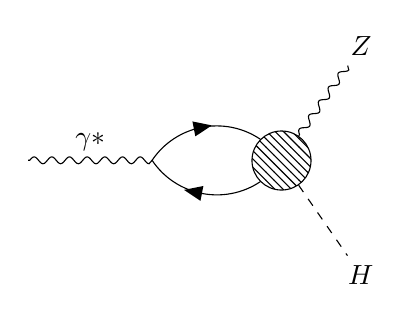
\begin{tikzpicture}[baseline=(g2.base)]
		\begin{feynman}
			\diagram[horizontal=g1 to g2]{
			g1 --[photon, edge label=\(\gamma*\)] g2;
			g2 --[fermion,quarter left] t1[blob];
			g2 --[anti fermion,quarter right] t1;
			t1 --[boson] z[particle=\(Z\)];
			t1 --[scalar] h[particle=\(H\)];
			};
		\end{feynman}
	\end{tikzpicture}
\end{align*}
Simply put, once we can arrive at a top bubble as in the second diagram in the beginning after nonrelativistic approximation, this top bubble can be replaced by $G(0,0 ; E)$.

To the lowest order of those couplings between top quarks and external lines, we're considering
\begin{align*}
	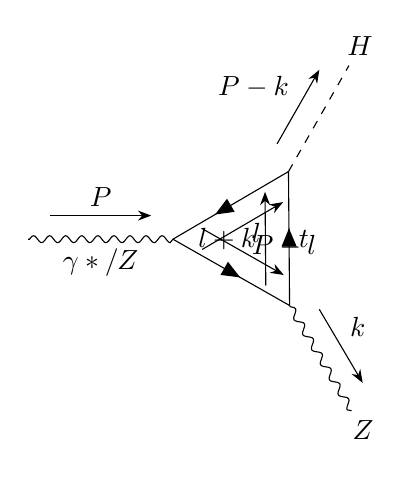
\begin{tikzpicture}[baseline=(g2.base)]
		\begin{feynman}
			\diagram[horizontal=g1 to g2]{
			% e1[particle=\(e^-\)] --[fermion] g1 --[fermion] e2[particle=\(e^+\)];
			g1 --[photon, edge label'=\(\gamma*/Z\),momentum=\(P\)] g2;
			g2 --[fermion,momentum=\(l\)] t1 --[boson,momentum=\(k\)] z[particle=\(Z\)];
			g2 --[anti fermion,momentum'=\(P-l\)] t2 --[scalar,momentum=\(P-k\)] h[particle=\(H\)];
			t1 --[fermion,edge label'=\(t\),momentum=\(l+k\)] t2;
			};
		\end{feynman}
	\end{tikzpicture}
	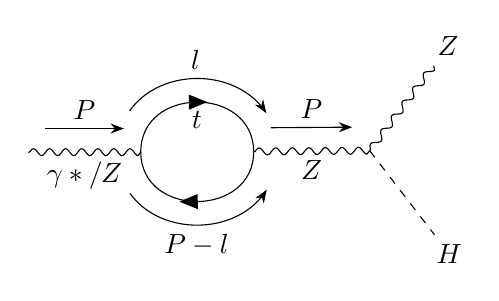
\begin{tikzpicture}[baseline=(g2.base)]
		\begin{feynman}
			\diagram[horizontal=g1 to g2]{
			% e1[particle=\(e^-\)] --[fermion] g1 --[fermion] e2[particle=\(e^+\)];
			g1 --[photon, edge label'=\(\gamma*/Z\),momentum=\(P\)] g2;
			g2 --[fermion, half left, edge label'=\(t\),momentum=\(l\)] t1 --[boson,momentum=\(P\),edge label'=\(Z\)] z1;
			g2 --[anti fermion, half right,momentum'=\(P-l\)] t1 --[draw=none] z1;
			z1 --[scalar] h[particle=\(H\)];
			z1 --[boson] z[particle=\(Z\)];
			};
		\end{feynman}
	\end{tikzpicture}
\end{align*}
The second one is well-discussed in \cite{Beneke:2013jia}. Beneke et al. gave the explicit relation between the Coulomb Green function and the total cross section via optical theorem
\begin{align}
	\begin{aligned} \Pi_{\mu \nu}^{(X)}\left(q^{2}\right) &=i \int d^{4} x e^{i q \cdot x}\left\langle 0\left|T\left(j_{\mu}^{(X)}(x) j_{\nu}^{(X)}(0)\right)\right| 0\right\rangle \\ &=\left(q_{\mu} q_{\nu}-q^{2} g_{\mu \nu}\right) \Pi^{(X)}\left(q^{2}\right)+q_{\mu} q_{\nu} \Pi_{L}^{(X)}\left(q^{2}\right) \end{aligned}
\end{align}
where the vector current $j_{\mu}^{(v)}=\bar{t} \gamma_{\mu} t$ and the axial vector current $j_{\mu}^{(v)}=\bar{t} \gamma_{\mu}\gamma_5 t$
\begin{align}
	\begin{aligned} \sigma_{t \bar{t} X}=\sigma_{0} \times 12 \pi \operatorname{Im}[& e_{t}^{2} \Pi^{(v)}\left(q^{2}\right)-\frac{2 q^{2}}{q^{2}-M_{Z}^{2}} v_{e} v_{t} e_{t} \Pi^{(v)}\left(q^{2}\right) \\ &\left.+\left(\frac{q^{2}}{q^{2}-M_{Z}^{2}}\right)^{2}\left(v_{e}^{2}+a_{e}^{2}\right)\left(v_{t}^{2} \Pi^{(v)}\left(q^{2}\right)+a_{t}^{2} \Pi^{(a)}\left(q^{2}\right)\right)\right] \end{aligned}
\end{align}
However, we can directly access the amplitude. Here we hold all conventions of signs implicitly as $\eta$\cite{Romao:2012pq}. 

The amplitude of the second diagram is 
\begin{align}
	&\bar u(p_1)\pqty{-i\eta_ee\gamma_{\mu}}u(p_2)\frac{-ig^{\mu\nu}}{P^2+i0}\tr\Bqty{(-i\eta_eeQ_t\gamma_{\nu})\frac{1+\gamma^0}{2}\notag\\&\pqty{-i\eta\eta_Z\frac{g}{\cos\theta_W}\gamma_\rho\pqty{g_V^t-g_A^t\gamma^5}}\frac{1-\gamma^0}{2}}\frac{-ig^{\rho\sigma}}{P^2-M_Z^2+i0}\frac{igm_Zg_{\sigma\omega}}{\cos\theta_W}\epsilon^{\omega}(k)
\end{align}

We'll start to expand the first diagram. The triangle loop is expressed as
\begin{align}
	-\int\mmd[d]{l}\tr\left\{\pqty{-i\eta_eeQ_t\gamma_{\mu}}\frac{i\pqty{\slashed P-\slashed l+m_t}}{(P-l)^2-m_t^2+im_t\Gamma_t}\pqty{-i\frac{g}{2}\frac{m_t}{m_W}}\frac{i\pqty{\slashed l+\slashed k+m_t}}{(l+k)^2-m_t^2+im_t\Gamma_t}\right.\notag\\\left.\pqty{-i\eta\eta_Z\frac{g}{\cos\theta_W}\gamma_\nu\pqty{g_V^t-g_A^t\gamma^5}}\frac{i\pqty{\slashed l +m_t}}{l^2-m_t^2+{im_t\Gamma_t}}\right\}
\end{align}
We have the following regions
\begin{align}
	\begin{aligned}
		\operatorname{hard}(\mathrm{h}) :        & \ell^{0} \sim m, \quad   &   & \ell \sim m       \\
		\operatorname{soft}(\mathrm{s}) :        & \ell^{0} \sim m v, \quad &   & \ell \sim m v     \\
		\operatorname{potential }(\mathrm{p}) :  & \ell^{0}   \sim m v^{2}, &   & \ell \sim m v     \\
		\operatorname{ultrasoft }(\mathrm{us}) : & \ell^{0}  \sim m v^{2},  &   & \ell \sim m v^{2}
	\end{aligned}
\end{align}
and $P=(2m_t+E,\vb{0})\sim (m_t+m_tv^2,0)$, $k\sim(m_t,m_t)$. We're to put the loop momentum in potential region. The propagators in the integrand is then simplified to (with a shift in $l^0\to m_t+\epsilon$)
\begin{align}
	\frac{i\pqty{\slashed l +m_t}}{l^2-m_t^2+{im_t\Gamma_t}}=\frac{i\pqty{\pqty{m_t+\epsilon}\gamma^0+l^i\gamma_i+m_t}}{\pqty{m_t+\epsilon}^2-\vb{l}^2-m_t^2+im_t\Gamma_t}\to \frac{1+\gamma^0}{2}\frac{i}{\epsilon-\frac{\vb{l}^2}{2m_t}+\frac{i\Gamma_t}{2}}
\end{align}
\begin{align}
	\frac{i\pqty{\slashed l-\slashed P+m_t}}{(P-l)^2-m_t^2+im_t\Gamma_t}&=\frac{i\pqty{\pqty{m_t+\epsilon-2m_t-E}\gamma^0+l^i\gamma_i+m_t}}{\pqty{2m_t+E-m_t-\epsilon}^2-\vb{l}^2-m_t^2+im_t\Gamma_t}\\&=\frac{i\pqty{\pqty{\epsilon-m_t-E}\gamma^0-l^i\gamma_i+m_t}}{\pqty{m_t+E-\epsilon}^2-\vb{l}^2-m_t^2+im_t\Gamma_t}\to \frac{1-\gamma^0}{2}\frac{i}{E-\epsilon-\frac{\vb{l}^2}{2m_t}+\frac{i\Gamma_t}{2}}
\end{align}
\begin{align}
	\frac{i\pqty{\slashed l+\slashed k+m_t}}{(l+k)^2-m_t^2+im_t\Gamma_t}=\frac{i\pqty{\pqty{m_t+\epsilon+k^0}\gamma^0+(l^i+k^i)\gamma_i+m_t}}{\pqty{m_t+\epsilon+k^0}^2-(\vb{l}+\vb{k})^2-m_t^2+im_t\Gamma_t}\to \frac{i\pqty{\slashed{\tilde{k}}+m_t}}{\tilde{k}^2-m_t^2+im_t\Gamma_t}
\end{align}
where $\tilde{k}=(k^0+m_t,\vb{k})$. To calculate the amplitude, a more appropriate way is to define a substitution rule for the top loop. We already know that in leading power
\begin{align}
	G(E)&=\int \frac{\dd^{d-1} \mathbf{p}}{(2 \pi)^{d-1}} \frac{\dd^{d-1} \mathbf{p}^{\prime}}{(2 \pi)^{d-1}}\frac{-(2 \pi)^{d-1} \delta^{(d-1)}\left(\mathbf{p}^{\prime}-\mathbf{p}\right)}{E+i \epsilon-\frac{\mathbf{p}^{2}}{m}}\xrightarrow{\epsilon\to\Gamma_t}\int\mmd[d-1]{l}\frac{-1}{E-\frac{\vb{l}^2}{m_t}+i\Gamma_t}\\&=i\int\mmd[d]{l}\frac{i}{\epsilon-\frac{\vb{l}^2}{2m_t}+\frac{i\Gamma_t}{2}}\frac{i}{E-\epsilon-\frac{\vb{l}^2}{2m_t}+\frac{i\Gamma_t}{2}}
\end{align}
For the top bubble type diagram
\begin{align*}
	\int\mmd{l}\frac{i\pqty{\slashed l-\slashed P+m_t}}{(P-l)^2-m_t^2+im_t\Gamma_t}\Gamma\frac{i\pqty{\slashed l +m_t}}{l^2-m_t^2+{im_t\Gamma_t}}\to\frac{1-\gamma^0}{2}\Gamma\frac{1+\gamma^0}{2}iG(E)
\end{align*}
where $\Gamma$ is arbitrary coupling sandwiched between two top propagators. 

For the top triangle diagram
\begin{align*}
	\int\mmd{l}\frac{i\pqty{\slashed l-\slashed P+m_t}}{(P-l)^2-m_t^2+im_t\Gamma_t}\Gamma_1\frac{i\pqty{\slashed l+\slashed k+m_t}}{(l+k)^2-m_t^2+im_t\Gamma_t}\Gamma_2\frac{i\pqty{\slashed l +m_t}}{l^2-m_t^2+{im_t\Gamma_t}}\\\to\frac{1-\gamma^0}{2}\Gamma_1\frac{i\pqty{\slashed{\tilde{k}}+m_t}}{\tilde{k}^2-m_t^2+im_t\Gamma_t}\Gamma_2\frac{1+\gamma^0}{2}iG(E)
\end{align*}


\section{One Loop Subtraction and the Determination of the Renormalization Artifact}
To get the exact contribution from Coulomb gluon exchanges and to avoid double counting, one must calculate the following diagram: 
\begin{align}
	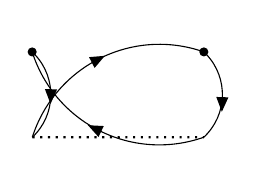
\begin{tikzpicture}[baseline=(a.base)]
		\begin{feynman}
			\diagram[small,horizontal=a to b]{
				a[dot] --[quarter left, fermion] o1 --[quarter left, fermion] b[dot];
				a --[quarter right, anti fermion] o2 --[quarter right, anti fermion] b;
			};
			\diagram*{
				(o1) --[ghost] (o2);
			};
		\end{feynman}
	\end{tikzpicture}
\end{align}
and the full amplitude with this correction is obtained via replacing the leading order one. 
\begin{align}
	&\mu^{2(3-d)}\int\mmd[d-1]{l_1}\mmd[d-1]{l_2}\frac{1}{E-\frac{\vb{l}_1^2}{m_t}+i\Gamma_t}\frac{1}{E-\frac{\vb{l}_2^2}{m_t}+i\Gamma_t}\frac{1}{\pqty{\vb{l}_1-\vb{l}_2}^2}\\
	&=-\frac{m_t^2}{32 \pi ^2 (d-3)}-\frac{m_t^2 (\log (-m_t (E+i \Gamma ))-2 \log (\mu )+\gamma_E -1-\log (\pi ))}{32 \pi ^2}+O\left(d-3\right)
\end{align}
Multiply the coupling $-g_s^2C_F=-\frac{16\pi\alpha_s}{3}$, the first logarithm is exactly what appears in \eqref{G} in this order (with an extra $-2\log{m}$ term to fix the dimension in the logarithm, in \cite{Melnikov:1994jb} they appears to have chosen a scheme with no $\mu$ presence). Now based on which scheme we choose, we may now determine the renormalization artifact $D$ and subtract the one loop level Coulomb contribution in the full QCD calculation to avoid double counting. 

\appendix
\section{Pseudoscalar Higgs Decay}

\section{$\gamma*\to ZH$}
We then have an overall factor\footnote{Convention follows \cite{Romao:2012pq}. One only needs to check the sign convention $\eta$. }
\begin{align}
	&-\tr{\pqty{-i\eta_eeQ_t\gamma^{\mu}}\frac{1-\gamma^0}{2}\pqty{-i\frac{g}{2}\frac{m_t}{m_W}}\frac{i\pqty{\slashed{\tilde{k}}+m_t}}{\tilde{k}^2-m_t^2+im_t\Gamma_t}\pqty{-i\eta\eta_Z\frac{g}{\cos\theta_W}\gamma^{\nu}\pqty{g_V^t-g_A^t\gamma^5}}\frac{1+\gamma^0}{2}}\notag\\
	&=-\pqty{-i\eta_eeQ_t}\pqty{-i\frac{g}{2}\frac{m_t}{m_W}}\frac{i}{\tilde{k}^2-m_t^2+im_t\Gamma_t}\pqty{-i\eta\eta_Z\frac{g}{\cos\theta_W}}\notag\\&\pushright{\tr{\gamma^{\mu}\frac{1-\gamma^0}{2}\pqty{\slashed{\tilde{k}}+m_t}\gamma^{\nu}\pqty{g_V^t-g_A^t\gamma^5}\frac{1+\gamma^0}{2}}}\notag\\
	&=\frac{g^2m_t}{2m_W\cos\theta_W}\frac{\eta\eta_Z\eta_eeQ_t}{\tilde{k}^2-m_t^2+im_t\Gamma_t}\tr{\gamma^{\mu}\frac{1-\gamma^0}{2}\pqty{\slashed{\tilde{k}}+m_t}\gamma^{\nu}\pqty{g_V^t-g_A^t\gamma^5}\frac{1+\gamma^0}{2}}\notag\\
	&=\frac{g^2m_t}{2m_W\cos\theta_W}\frac{\eta\eta_Z\eta_eeQ_t}{\tilde{k}^2-m_t^2+im_t\Gamma_t}\tr{\gamma^{\mu}\frac{1-\gamma^0}{2}\pqty{\slashed{\tilde{k}}+m_t}\gamma^{\nu}\pqty{g_V^t-g_A^t\gamma^5}}\notag\\
	&=\frac{g^2m_t}{m_W\cos\theta_W}\frac{\eta\eta_Z\eta_eeQ_t}{\tilde{k}^2-m_t^2+im_t\Gamma_t} \left(-g_V^t g^{0 \mu } \tilde{k}^{\nu }+g_V^t g^{0 \nu } \tilde{k}^{\mu }-g_V^t \tilde{k}^0 g^{\mu  \nu }+g_V^t m_t g^{\mu  \nu }-i g_A^t \epsilon ^{0 \mu  \nu  \rho}\tilde{k}_{\rho}\right)
\end{align}
% TODO: add Z boson intermidiating diagram
Considering the external states, applying Feynman gauge, and counting the electron-positron pair in, we have
\begin{align}
	&\frac{g^2m_t}{m_W\cos\theta_W}\frac{\eta\eta_Z\eta_eeQ_t}{\tilde{k}^2-m_t^2+im_t\Gamma_t} \left(-g_V^t g^{0 \mu } \tilde{k}^{\nu }+g_V^t g^{0 \nu } \tilde{k}^{\mu }-g_V^t \tilde{k}^0 g^{\mu  \nu }+g_V^t m_t g^{\mu  \nu }-i g_A^t \epsilon ^{0 \mu  \nu  \rho}\tilde{k}_{\rho}\right)\notag\\&\pushright{\epsilon_{\nu}(k)\frac{-i}{P^2+i0}\bar{u}(p_1)\pqty{-ie\gamma_{\mu}}u(p_2)}\notag\\
	&=\frac{g^2m_t}{m_W\cos\theta_W}\frac{\eta\eta_Z\eta_eeQ_t}{\tilde{k}^2-m_t^2+im_t\Gamma_t}\frac{-i}{P^2+i0}\pqty{-ie} \notag\\&\pushright{\bar{u}(p_1)\left(-g_V^t \gamma^{0} m_t\epsilon^0(k)+g_V^t \epsilon^0(k) \slashed{\tilde{k}}-g_V^t \tilde{k}^0 \slashed\epsilon(k)+g_V^t m_t \slashed\epsilon(k)-i g_A^t \epsilon ^{0 \mu  \nu  \rho}\tilde{k}_{\rho}\gamma_{\mu}\epsilon_\nu(k)\right)u(p_2)}\notag\\
	&=\frac{g^2m_t\pqty{-ie}}{m_W\cos\theta_W}\frac{\eta\eta_Z\eta_eeQ_t}{\tilde{k}^2-m_t^2+im_t\Gamma_t}\frac{-i}{P^2+i0} \bar{u}(p_1)\left(g_V^t \epsilon^0(k) \slashed{{k}}-g_V^t {k}^0 \slashed\epsilon(k)-i g_A^t \epsilon ^{0 \mu  \nu  \rho}\tilde{k}_{\rho}\gamma_{\mu}\epsilon_\nu(k)\right)u(p_2)
\end{align}
The loop part is 
\begin{align}
	\int\mmd[d]{l}\frac{i}{\epsilon-\frac{\vb{l}^2}{2m_t}+\frac{i\Gamma_t}{2}}\frac{i}{E-\epsilon-\frac{\vb{l}^2}{2m_t}+\frac{i\Gamma_t}{2}}=\int\mmd[d-1]{l}\frac{i}{E-\frac{\vb{l}^2}{m_t}+i\Gamma_t}
\end{align}
and this is the leading order of $G(E)$, differed by a overall sign. While this integral is divergent in 3-dimension, by integrating it in $(d-1)$-dimension then take the limit, the divergence disappeared and the result in \eqref{G} is obtained. 

\begin{acknowledgments}

\end{acknowledgments}

\appendix

\bibliography{../Bib}
% \begin{thebibliography}{10}

% \end{thebibliography}


\end{document}



